%!TEX root = ../dissertation.tex
\begin{savequote}[75mm]
	You cannot kill the truth. You cannot kill justice. You cannot kill what we are fighting for.
	\qauthor{Jean Dominique, Haitian democracy activist.}
\end{savequote}

\chapter{Metodologia}
\label{chap:metodologia}

In questo capitolo analizzeremo lo studio di Amnesty International "Il Barometro dell'Odio" che ha fornito il database originario, già in gran parte codificato, che è stato utilizzato per le nostre analisi nel presente lavoro. In seguito vedremo le ulteriori elaborazioni fatte da noi specificamente per questa tesi, discutendone gli aspetti metodologici.

\section{Il Barometro dell'Odio}

\subsection{Amnesty International e il Tavolo per il contrasto ai discorsi d’odio}
Le analisi de "Il Barometro dell'Odio" \footnotetext{\url{https://www.amnesty.it/campagne/contrasto-allhate-speech-online/}} fanno parte di "Contrasto all’hate speech online", una delle 12 campagne attualmente portate avanti da Amnesty International. Oltre alla ricerca, questa campagna comprende una Task Force "Hate Speech" per la creazione di contro-narra-zione sul tema, un videogioco rivolto alla sensibilizzazione dei più giovani chiamato "HateSick” e svariate attività educative per le scuole e per la formazione professionale. Questa articolata iniziativa nasce per rispondere al problema dell'odio online definito, sulla stessa pagina web della campagna, come \textit{diffuso}, poiché coinvolge molti utenti come vittime o colpevoli, \textit{liquido}, perchè si propaga ed è difficile da contenere e \textit{pericoloso} perché è causa ed effetto del cambiamento culturale che può portare a discriminazioni anche offline.
\begin{wrapfigure}{r}{5cm}
	\fcolorbox{black}{yellow}{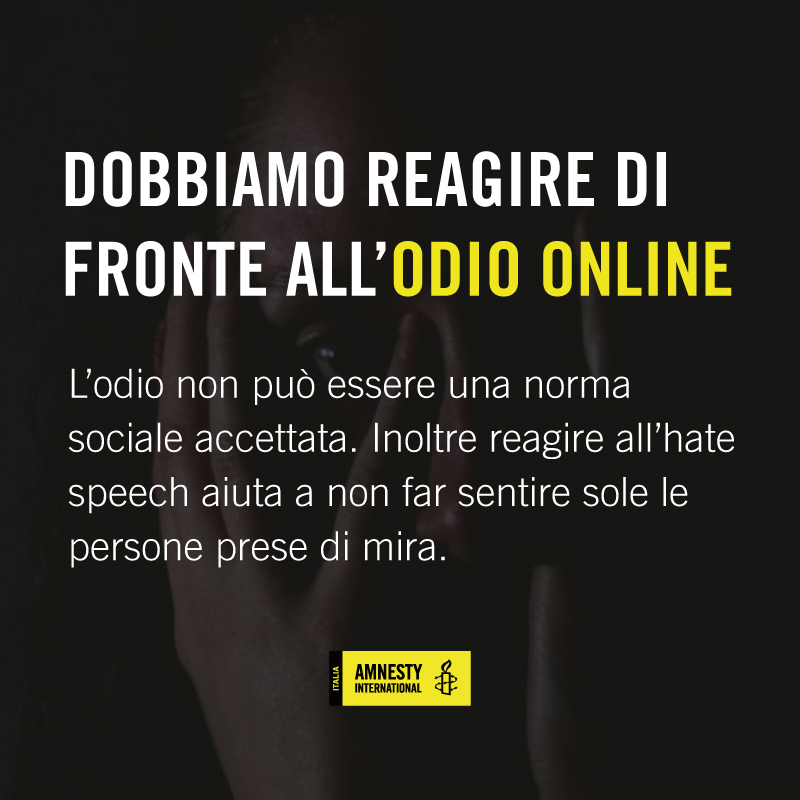
\includegraphics[width=5.5cm]{figures/3}}   
	\caption{Una delle cartoline prodotte da Amnesty International Italia contenuta all'interno del "Kit per contrastare l'\textit{hate speech}"}
	\label{3}
\end{wrapfigure}

Oltre ad aver elaborato una serie di precise richieste ai social media, agli stati europei e alle autorità italiane, questa campagna di Amnesty international ha scritto creato un vademecum destinato ai singoli cittadini, affinché ognun* possa fare qualcosa per contrastare questo fenomeno [Fig.~\ref{3}]. \footnotetext{\url{https://www.amnesty.it/aiutaci-a-contrastare-lodio-online/}}

Anche grazie a questo progetto, è nata la "Rete nazionale per il contrasto ai discorsi e ai fenomeni d’odio", un importante gruppo di associazioni e università (tra cui quella di Padova) [Fig. \ref{fig:rete}] che coinvolge giornalist*, avvocat*, scienziat* e attivist* da tutta Italia, con l'obiettivo di ridurre i fenomeni d'odio tramite la ricerca, azioni di \textit{advocacy} e \textit{lobby}, la condivisione di buone pratiche, la promozione di percorsi educativi e, ovviamente, la sensibilizzazione e la mobilitazione della società civile.

Il Barometro dell'Odio consiste in un monitoraggio costante di diversi social network. A partire dalle elezioni del 2018, periodicamente Amnesty International ha coinvolto centinaia di attivisti e decine di ricercator* e attivist* nell’aggregazione e nell'analisi di dati quantitativi e qualitativi che testimoniano la gravità dell’\textit{hate speech} online e ne individuano i bersagli principali.
\begin{figure}
	\fcolorbox{black}{yellow}{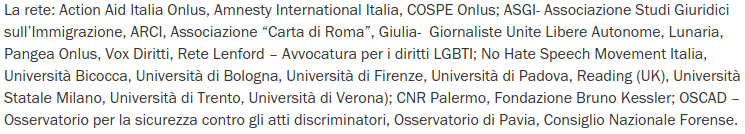
\includegraphics[width=\textwidth]{figures/rete}}
	\caption{Le realtà fondatrici della "Rete nazionale per il contrasto ai discorsi e ai fenomeni d’odio".}
	\label{fig:rete}
\end{figure}

Per ogni studio svolto vengono pubblicati tre documenti: una pagina sul sito dell'asso-ciazione con i grafici e i risultati principali; un articolo a cura dei e delle scienziat* che partecipano al "Tavolo per il contrasto ai discorsi d’odio", con tutte le analisi svolte e le evidenze che hanno fatto emergere, e una nota metodologica. I documenti prodotti riguardo allo studio sulle elezioni europee del 2019, che ha fornito i dati di partenza per la presente ricerca, verranno descritti qui di seguito (rispettivamente \citep{sito}, \citep{rapporto}, \citep{nota}).


\subsection{La raccolta dati}
Amnesty International Italia ha monitorato per 40  giorni  (dal  15  aprile fino alla conclusione della campagna elettorale il 24 maggio 2019) i profili Facebook e Twitter dei candidati al Parlamento europeo più attivi online e quelli dei leader di partito ai quali i candidati facevano riferimento. Sono stati raccolti in un primo momento oltre 4 milioni e 250 mila di contenuti dai \textit{feed} dei profili dei politici, ne sono poi stati selezionati 100 mila per l'analisi rispettando alcune proporzioni che vedremo tra poco [Fig. \ref{fig:barometro}]. Non si conoscono, a oggi, rilevazioni – né in Italia né in altri paesi dell’Unione Europea – così estese rispetto alla campagna delle scorse elezioni per il rinnovo del Parlamento europeo. La particolarità di questa raccolta sta nel considerare contemporaneamente sia le campagne politiche (cioè i post prodotti dai candidati), sia le reazioni sviluppate dagli utenti nei commenti. La finestra della raccolta dei commenti e delle statistiche di viralità dei post è stata estesa fino al 31 maggio per comprendere anche le interazioni con i contenuti postati dai candidati a fine campagna. Per la raccolta sono state utilizzate le \textit{Application Programming Interface} (API) ufficiali dei due social network, con l'unica limitazione nel caso di Twitter di non poter avere accesso a \textit{tutti} i contenuti, ma solo ad una selezione casuale di essi. Essendo i commenti analizzati nello studio un campionamento altrettanto casuale di quelli raccolti, questa limitazione non costituisce un problema metodologico. Le API di Facebook sono invece limitate ad un massimo di 24 commenti per post, caso riscontrato solo in pochi contenuti analizzati in questo studio, non riducendo significativamente, quindi, la rappresentatività del campione.
\begin{figure}
	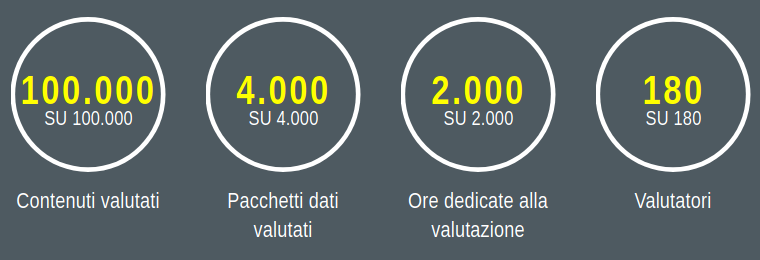
\includegraphics[width=\textwidth]{figures/barometro}
	\caption{Alcune statistiche riassuntive dei risultati dello studio Il Barometro dell'Odio, pubblicate su www.amnesty.it/cosa-facciamo/elezioni-europee/.}
	\label{fig:barometro}
\end{figure}

Sono stati presi in considerazione i 40 politici più attivi su Twitter, e i 40 più attivi su Facebook in base alla semplice somma del numero di tweet/post pubblicati con il relativo numero di risposte/commenti ricevuti.
Per assicurare un’equa rappresentazione degli schieramenti e del territorio, sono stati valutati i \textit{feed} raccolti dai 4 politici complessivamente più attivi per ogni lista e il \textit{feed} di almeno un rappresentante di ogni circoscrizione per lista. Inoltre, per ogni lista sono stati presi in considerazione almeno una donna e almeno un uomo. A seguito della pubblicazione dei risultati delle elezioni sono stati introdotti nel campione altri candidati eletti e non precedentemente considerati. Il risultato consiste in un campione di 77 politici che, oltre a essere stati monitorati, sono stati anche valutati. Sui 27.009 post/tweet raccolti per questi politici ne sono stati valutati l'80\% (21.596). Successivamente sono stati selezionati in modo casuale un numero di commenti proporzionato al totale dei commenti ricevuti per ogni post/tweet, partendo da un minimo di 4 e raggiungendo i 2-3mila commenti per post con 100mila commenti totali.

\subsection{La valutazione dei contenuti}
Circa 180 attivisti di Amnesty International Italia sono stati istruiti su come svolgere la valutazione dei contenuti e hanno realizzato il lavoro tramite il sito shinyapps.io in cui venivano assegnati, in modo casuale, una serie di pacchetti da 50 contenuti da valutare. Nell'applicazione è stato mostrato il contenuto testuale; il nome del politico dal cui \textit{feed} proveniva il contenuto; la distinzione tra tweet/post e risposta/commento; nel  caso di  risposta/commento, è stato mostrato il  tweet/post in replica al  quale il contenuto era stato pubblicato.

Per ogni contenuto sono stati valutati: il tema (donne, lgbti, disabilità,migranti rifugiati e persone con background migratorio, rom, minoranze religiose,solidarietà, povertà socio-economica, altro); l'accezione (negativa, positiva); se negativa la tipologia (non problematico, problematico, \textit{hate speech}, ambiguo); se problematico o \textit{hate speech} il target (il politico autore del contenuto, un altro politico, l'autore del commento/risposta precedente, un singolo individuo o un gruppo perché riconducibile a una categoria soggetta a discriminazione, altro); la categoria del  target (donne, lgbti,  persone  con  disabilità, migranti rifugiati e persone con  background migratorio, rom, musulmani, ebrei, un singolo o  un gruppo per lo svolgimento di attività di tipo umanitario e/o solidaristico, persone in condizione di  povertà socio-economica, non  riconducibile ad  alcuna categoria/altro).
Per la definizione di \textit{hate speech} si è utilizzata quella contenuta nella Raccomandazione di politica generale n.15  dell'ECRI relativa alla lotta contro il discorso d'odio (adottata l'8 dicembre 2015) \citep{ecri2015}, già citata del capitolo "\nameref{chap:hate}".

Ogni contenuto è stato valutato da tre valutatori diversi; se le tre valutazioni sono risultate essere coerenti sono state accettate. I contenuti di \textit{hate speech}, quelli ritenuti ambigui da almeno due valutatori e quelli per i quali non c’era allineamento tra i tre valutatori, sono stati rivisti da esperti appartenenti al Tavolo per il Contrasto ai Discorsi d’Odio.

\subsection{Le elezioni europee del 2019}
Prima di affrontare i riusultati dello studio, un breve approfondimento sulle elezioni europee e sui risultati dei partiti italiano a questa tornata del 2019.
Le elezioni europe assumono una rilevanza secondaria rispetto a quelle nazionali ed hanno caratteristiche proprie come, ad esempio, una minore affluenza complessiva e risultati meno significativi per i partiti in quel momento al governo, dovuti al "voto di protesta" che  in questo tipo di elezioni è più presente \citep{reif1980}. Vengono quindi definite "second-order elections", anche in funzione del fatto che prevedono budget molto più limitati per la campagna elettorale che in generale dura meno rispetto alle elezioni nazionali.
Questo tipo di elezioni concentra le sue tematiche su due filoni principali: quello della politica interna e degli effetti del voto sugli assetti nazionali e la discussione (spesso minoritaria) sulle questioni effettivamente europee. Negli ultimi anni, sempre di più, si è passati a discutere della legittimità del sistema europeo, soprattutto in relazione ai temi della migrazione e a quello dell'\textit{austerity} imposta ad alcuni paesi dopo la crisi del 2008. Anche nella tornata elettorale del 2019 si sono creati due evidenti schieramenti: uno euroscettico e l'altro europeista, dando maggiore rilievo alla discussione su contenuti sovranazionali. Questo tipo di opinioni contrastanti ha cambiato il posizionamento dei principali partiti nei vari paesi dell'unione e l'equilibrio tra di essi \citep{meijers2017}, con effetti importanti anche in Italia, dove  almeno uno dei partiti in quel momento al governo ha fatto una campagna dichiaratamente anti-europeista. Se nel 2009 solo il 20\% dell'elettorato ha votato partiti antieuropeisti, nel 2014 si è arrivati a superare il 50\% e nel 2019 è stato addirittura raggiunto il 58\%, \citep{seddone2019}. Nella figura \ref{fig:europee} possiamo vedere i risultati delle elezioni e le tendenze dei cinque principali partiti.
\begin{figure}
	\centering
	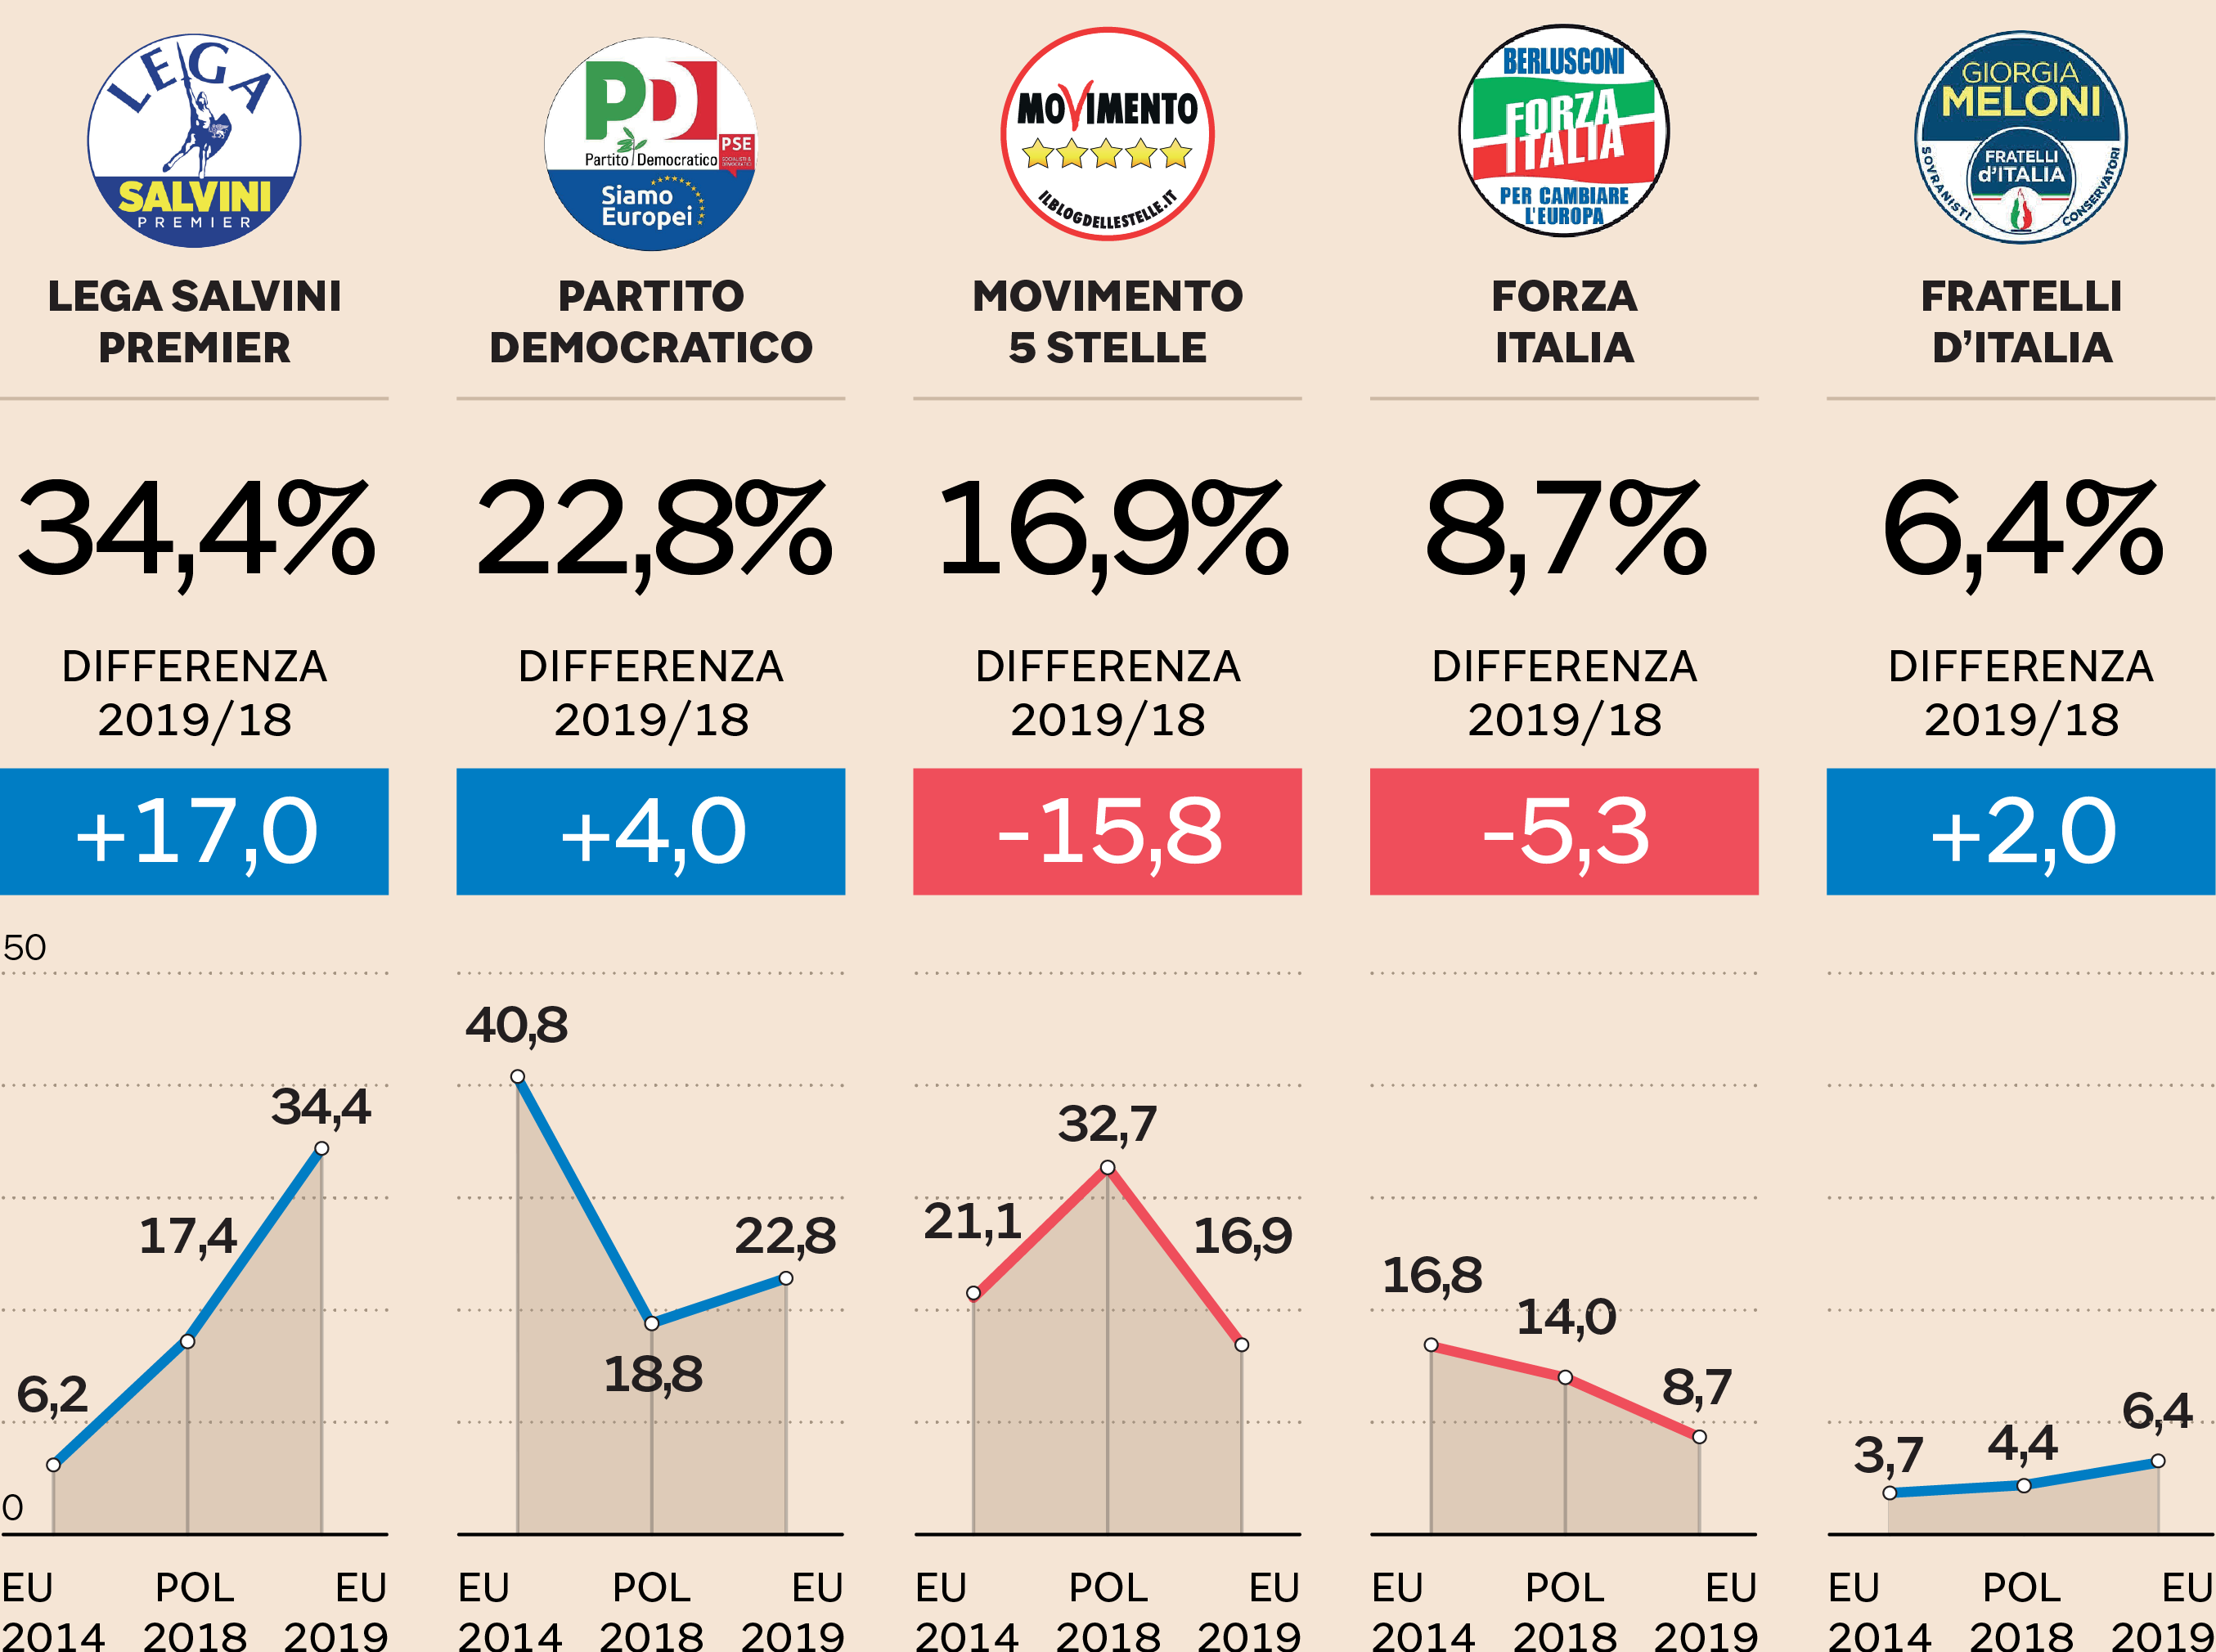
\includegraphics[width=0.6\textwidth]{figures/europee}
	\caption{I risultati delle elezioni europee del 2019 in Italia, con confronti con le precedenti due elezioni. Infografica pubblicata da Weeklymagazine.it}
	\label{fig:europee}
\end{figure}


\subsection{I risultati del Barometro}
I due principali risultati di questa ricerca da un punto di vista statistico riguardano l'effetto del tono dei politici e del tema da loro trattato sul tipo di commenti generati.
Risulta infatti confermato con significatività statistica che un tono negativo nei post dei politici (post codificati come negativi/problematici/\textit{hate speech}) sia in grado di generare più commenti negativi (negativi/problematici/\textit{hate speech}) rispetto a equivalenti post positivi e neutro. 
L'ipotesi riguardo i temi trattati nei post risulta parzialemente confermata: è stata riscontrata una significatività per i temi "immigrazione" e "minoranze religiose", ma non per quello riguardo il tema "donne", come supposto inizialmente [Fig. \ref{fig:amntarget}]. 
\begin{figure}
	\centering
	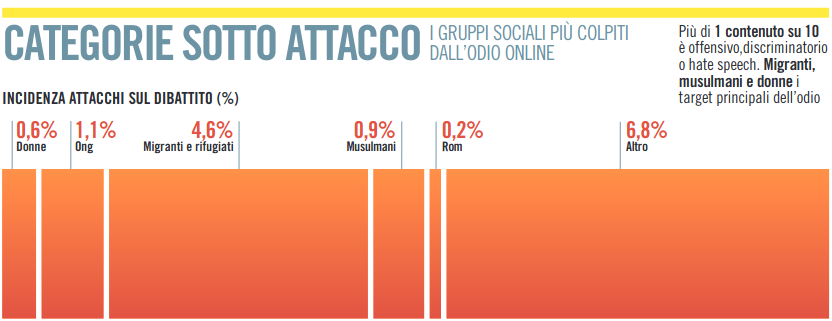
\includegraphics[width=\textwidth]{figures/amntarget}
	\caption{Incidenza delle categorie sotto attacco nei commenti. Immagine pubblicata nel report di Amnesty International sul "Barometro dell'odio: elezioni europee del 2019"}
	\label{fig:amntarget}
\end{figure}

Vengono inoltre proposte alcune considerazioni più generali riguardo proprio i temi toccati dalla campagna elettorale. Rispetto al precedente Barometro sulle elezioni politiche del 2018, gli attacchi rivolti a comunità migranti non si sono ridimensionate, ma si sono normalizzate passando anche ad attacchi alla solidarità e a chi la promuove. La discussione su questi argomenti risulta ancora più polarizzata, anche a causa dell'intreccio con il dibattito sull'Unione Europea.

Riguardo le categorie utilizzate per individuare i livelli di odio generali, risulta che l'11,5\% dei 100mila contenuti valutati sia risultato essere offensivo e/o discriminatorio o \textit{hate speech}. Limitandoci al solo \textit{hate speech} l'incidenza si attesta invece all'1\% del totale dei contenuti. Soffermandosi sui contenuti riguardo l'immigrazione (8\% del totale), il 42\% di questi risultano discriminatori o \textit{hate speech}, percentuale di poco inferiore solo a quella relativa al tema "minoranze religiose" che fa riscontrare il 47.5\% di messaggi offensivi e molto superiore alla media generale. 

Guardando solo ai 21.596 post/tweet dei politici valutati, solo 1 è stato etichettato come hatespeech (conteneva riferimenti alla “bonifica sociale e culturale” di un gruppo di persone rom). Tuttavia ben 415 post/tweet (quasi 2 su 100) sono stati ritenuti offensivi e/o discriminatori e tra questi sono molti quelli al limite dell’hate speech.

Non tutti i/le candidat* hanno utilizzato i social con uguale intensità ed efficacia: il 51,5\% delle interazioni totali è stata fatta registrare da Matteo Salvini. Gli altri esponenti seguono ad ampissima distanza e solo sei tra loro superano la soglia dell’1\%: Luigi Di Maio(14,5\%), Giorgia Meloni (8,3\%), Silvio Berlusconi (3,6\%), SilviaSardone (2,7\%) Carlo Calenda (1,7\%), Nicola Zingaretti (1,3\%) . Questo dato risulta interessente se comparato con quanto emerge dalla sezione “Report della Libreria inserzioni” pubblicata da Facebook in cui è possibile vedere quanto è stato speso dai singoli inserzionisti e, soprattutto, quali contenuti sono stati promossi. Nello studio di Amnesty International viene infatti riportato come Matteo Salvini sia stato il politico a spendere di più su questo social in pubblicità nel periodo considerato dallo studio, arrivando a  128.782 euro per la promozione di 58 post, alcuni dei quali successivamente codificati come problematici. Molti di questi sono inerenti al tema immigrazione: uno di questi pubblicizzava il video di una persona di origine straniera mentre littigava con un controllore su un treno. Sul video sono stati spesi tra i 10mila e i 50mila euro, riuscendo a raggiungere 1 milione di utenti e ottenendo 80mila likes (e reazioni in generale) e più di 22mila commenti. Questo video rappresenta un esempio chiaro dei temi e della viralità raggiunta dai contenuti del politico, andando a vedere i principali temi trattati e l'incidenza della negatività raggiunta, questo emerge chiaramente [Fig. \ref{fig:amnpol}]. Inoltre il leader della Lega ha sicuramente investito più di altri candidati sulla comunicazione social, ottenendo risultati nettamente migliori nella diffusione dei suoi contenuti.
\begin{figure}
	\centering
	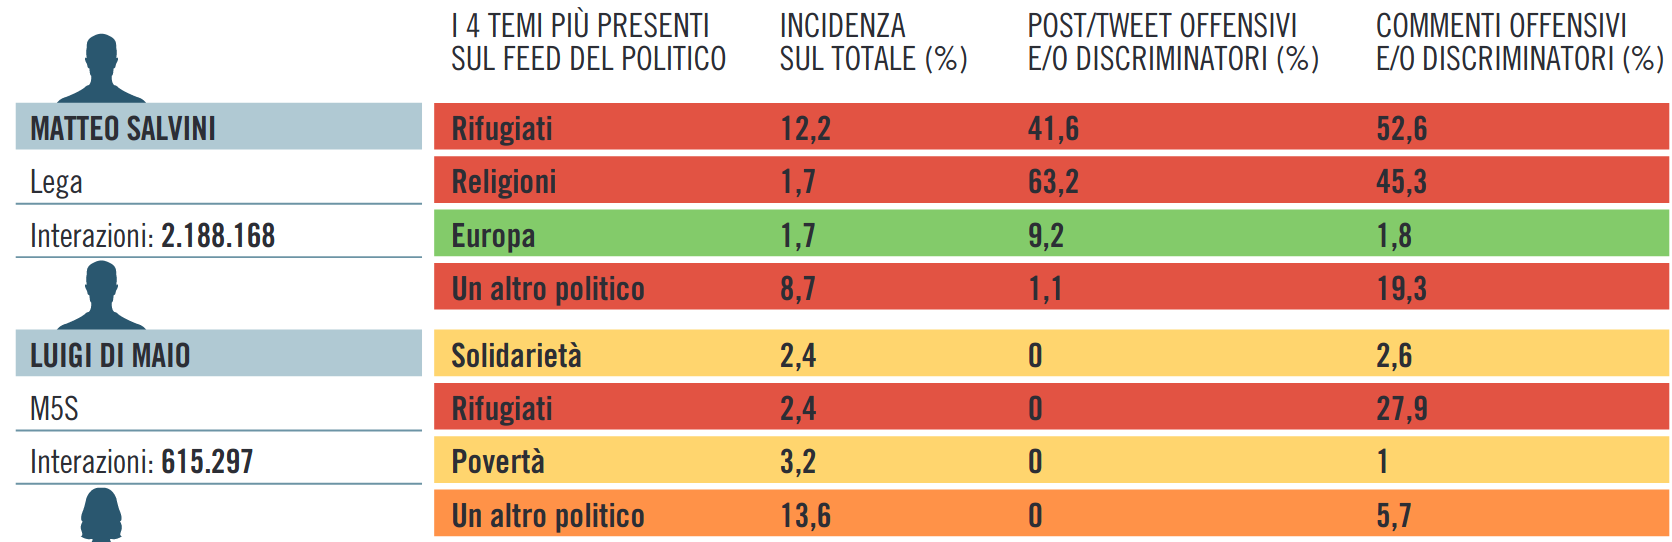
\includegraphics[width=\textwidth]{figures/amnpol}
	\caption{I temi più citati dai due politici con più interazioni (il tema "altro" non è stato preso in considerazione). I colori utilizzati indicano l’accezione prevalente del tema: verde per i contenuti con accezione negativa inferiori o uguali al 25\%, giallo tra il 26\% e il 50\%, arancione tra il 51\% e il 75\%, e rosso tra il 75\% e il 100\%. Immagine pubblicata nel report di Amnesty International sul "Barometro dell'odio: elezioni europee del 2019"}
	\label{fig:amnpol}
\end{figure}


\section{La codifica del \textit{Negative Campaign}}
A partire dai dati elaborati da Amnesty International, per il presente lavoro abbiamo provveduto alla ulteriore codifica di 10103 post e tweet di politici. Se infatti nel database originario erano presenti circa il doppio dei contenuti prodotti dai politici rispetto a quelli presi in considerazione in questa tesi, per metà di questi post non sono stati raccolti i relativi commenti. Inoltre alcuni commenti (circa 2 mila) non facevano riferimento a nessun post o tweet analizzato. Si arriva così all'utilizzo di 10103 post/tweet e di 78175 commenti, per un totale di 88278 contenuti utilizzati sui 100mila raccolti nel data base iniziale.
\begin{wrapfigure}{r}{7cm}
	
\includegraphics[width=\linewidth]{figures/neutro}
	\caption{Un post di campagna neutra, non ha infatti argomento politico.}
	\label{esempi1}
\end{wrapfigure}

La valutazione dei contenuti è stata possibile grazie alla preziosissima collaborazione di 9 persone con background accademico (Carlotta Baroni, Francesca Carotta, Giorgio Roda, Luigi Romano, Marilina Verna, Paola Biffi, Sara Vergolini, Samuele Maieron, Vanessa Bebi) che, dopo essere state opportunamente istruite, hanno codificato 2mila post di politici a testa. Ogni post, infatti, è stato codificato due volte da due valutat* all'oscuro del lavoro dei/delle collegh*. In caso di non accordo tra i \textit{coders}, il contenuto è poi stato rivisto per garantire omogeneità nell'interpretazione delle categorie anche nei casi più discutibili. L'accordo tra i due valutatori è stato comunque raggiunto nell’87\% dei casi.All'inizio del lavoro, dopo un incontro di formazione, è stata fornita ad ogni valutatore una scheda con le indicazioni per l'applicazione delle categorie, poi sono stati sottoposti a tutt* i/le valutat* gli stessi 500 contenuti, utilizzati come allenamento e come esempio. In seguito c'è stato un confronto collettivo sui dubbi emersi e sulle codifiche errate per garantire la massima omogeneità delle valutazioni. Il lavoro ha richiesto da 7 a 20 giorni di tempo, in base alla velocità di esecuzione delle varie persone che hanno partecipato.
\begin{wrapfigure}{r}{7cm}
	
\includegraphics[width=\linewidth]{figures/positivo}
	\caption{Un post di campagna positiva, si rimarca una proposta politica senza attaccare posizioni contrarie.}
	\label{esempi2}
\end{wrapfigure}

È stato analizzato solo il testo dei messaggi, non si è fatto, quindi, riferimento nè alle immagini nè ai link presenti nel post e nei tweet poiché la presente analisi voleva concentrarsi sul linguaggio dei politici, e in particolare sulle loro affermazioni, più che sui vari tipi di contenuti multimediali che i social media permettono di condividere.

Le categorie utilizzate per la valutazione sono state fondamentalmente due: la prima  prevedeva l'identificazione del tipo di campagna utilizzata nel post. Si poteva scegliere tra "neutro" quando il contenuto risultava impossibile da contestualizzare o quando non si riferiva a nessun tema politico; "positiva" quando veniva citata una propria proposta politica senza citare avversari politici o quando si promuoveva un proprio appuntamento elettorale; "comparativa" quando veniva citata una propria proposta e contemporaneamente quella rivale, ponendo in contrapposizione le due idee; "negativa" quando invece nessun riferimento alla propria idea veniva citata, ma si citavano posizioni o caratteristiche di altr*.
È stata quindi utilizzata una definizione puramente direzionale, che non comprendeva nessun aspetto valutativo del livello di negatività del contenuto analizzato.
\begin{figure}
	\centering
	
\includegraphics[width=\linewidth]{figures/negativapost}
	\caption{Un tweet di campagna negativa in cui non viene citata la propria proposta politica, ma si attacca solamente, in questo caso, un gruppo politico e un personaggio politico. Si fa riferimento a un consigliere di Casapoud accusato di stupro.}
	\label{esempi4}
\end{figure}

\begin{wrapfigure}{l}{9cm}
	
\includegraphics[width=\linewidth]{figures/comparativa}
	\caption{Un tweet di campagna comparativa, viene citata la propria tesi e comparata con quella di, in questo caso, un altro gruppo politico.}
	\label{esempi3}
\end{wrapfigure}
La seconda categoria utilizzata nelle valutazioni è stata applicata solo ai post classificabili come campagna "comparativa" o "negativa". In questi casi, è stato individuato il target (uno o massimo due) al quale faceva riferimento il contenuto del post/tweet. Le tipologie di target definite ex-ante, con cui classificare i contenuti valutati erano:  "privato cittadino" quando il post si riferiva a persone non note al pubblico e di cui non si conosceva il nome, come ad esempio, persone fotografate a manifestazioni o comparse in video diventati poi virali; "categoria di persone" quando veniva attaccata una categoria sociale o un gruppo in quanto tale, come per esempio la comunità rom o i "clandestini"; "personaggio pubblico" quando si faceva riferimento a una figura pubblica ma non di ambito politico come per esempio Roberto Saviano o un personaggio della TV; "personaggio politico" per persone impegnate in organizzazioni politiche oppure che ricoprivano, o avevano ricoperto in passato, cariche istituzionali di carattere politico; "gruppo non politico" per gruppi organizzati e riconosciuti in quanto tali come associazioni, ONG, ma anche aziende o associazioni di categoria come i giornalisti; "gruppo politico" per riferimenti a partiti, gruppi politici o schieramenti a tutti i livelli istituzionali. Nelle immagini [Figg. ~\ref{esempi1}, ~\ref{esempi2}, ~\ref{esempi3}, ~\ref{esempi4}] possiamo vedere alcuni esempi dei vari tipi di campagna elettorale e dei rispettivi target.


\section{Raccogliere \textit{Big Data}: le criticità delle API ufficiali}
Riguardo alla raccolta dati, una possibile criticità dello studio risiede nell'utilizzo delle API ufficiali, che restituiscono i contenuti delle piattaforme dopo che la \textit{content curation} è stata applicata dalle stesse. Questo significa che i post e tweet rimossi perchè non rispettosi delle \text{policy} dei social media, non vengono restituiti. È possibile che anche dei messaggi di \textit{hate speech} siano stati rimossi in modo automatizzato o manuale, non comparendo quindi nel database finale.
In generale, raccolte dati per studi indipendenti sulle piattaforme social risultano fragili se non basati su dati raccolti indipendentemente dalle piattaforme che si vogliono studiare ed eventualmente sottoporre a critica.
A seguito dello scandalo di Cambridge Analytica del 2018 (già citato nell'introduzione del presente lavoro), Facebook ha largamente ristretto i dati accessibili alle aziende e ai ricercatori, rendendo necessario un ripensamento complessivo dei \textit{computational methods} utilizzati fino a quel momento e portando alcuni studiosi ad interrogarsi sulla necessità di una "Computational Research in the Post-API Age" \citep{freelon2018}. Freelon, in particolare, ha riflettuto sulla necessità di utilizzare tecniche di \textit{scraping} per raccogliere questo tipo di dati e sulle possibili implicazioni giuridiche di queste tecniche che consistono fondamentalmente nel "raschiare" (dal verbo inglese \textit{scrape}) in modo automatizzato le pagine HTML dei social, estraendo in modo autonomo le informazioni di cui si ha bisogno dai \textit{document object model} (DOM) con cui sono organizzati i siti. Spesso è possibile però, che questa modalità di raccolta dati sia in violazione dei \textit{terms of service} (TOS) delle piattaforme.

Risulta importante anche rispettare i diritti degli/delle utenti di cui si analizzano i dati, conformandosi agli standard, per l'Europa, del \textit{General Data Protection Regulation} (GDPR). A proporre una riflessione su GDPR e TOS, e a proporre una conseguente soluzione tecnica sono, ad esempio, Mancosu e Vegetti \citep{mancosu2020}. Loro mettono in evidenza come le informazioni dei social, benché non più accessibili tramite API, rimangano comunque pubbliche e accessibili sul web. Hanno, quindi, elaborano un \textit{tool} semplice ed efficace per lo \textit{scraping} di profili Facebook.

Bernard Rider, già dal 2013, ha reso disponibile "Twitter Capture and Analysis Toolset" (DMI-TCAT), un software in grado di estrarre praticamente qualsiasi dato disponibile su Twitter tramite API ufficiali, ma registrando più volte al giorno i nuovi contenuti postati, evitando parte della moderazione del social. Nel 2014 ne discutono alcuni usi pratici e possibilità di ricerca \citep{bruns2014} poi largamente utilizzati negli anni successivi.

Soluzioni simili per Youtube, Amazon, Pornhub e Facebook sono state proposte dal collettivo Tracking Exposed di cui anch'io faccio parte
(\url{www.tracking.exposed}). Questi \textit{tool}, estensioni browser basate su JavaScript, compiono \textit{scraping} delle pagine social \textit{user-side}, e hanno permesso, tra le altre cose, l'analisi di elezioni nazionali italiane con metodologie innovative di analisi di questi \textit{new media} \citep{hargreaves2019} che non prevedono l'utilizzo di API ufficiali. Alcuni sperimentali comparazioni tra i dati registrati \textit{in vivo} tramite \textit{scraping} e le API ufficiali di Youtube \citep{yttrex2019}, hanno mostrato che il numero di video consigliati da Youtube che si ottengono tramite una richiesta all'API ufficiale differiscono da quelli raccolti utilizzando \textit{tools} di \textit{scraping}, sia con browser privi di cronologia pregressa che (ancora di più), con profili molto personalizzati, come si può vedere nell'immagine estratta dal report di workshop a cui ho partecipato nel 2019 durante la Summer School in Digital Methods dell'Università di Amsterdam [Fig. \ref{fig:api}]. Benchè Youtube sia molto diverso da altre piattaforme social, problemi simili potrebbero sorgere anche analizzando Facebook e Twitter.
\begin{figure}
	\fcolorbox{black}{red}{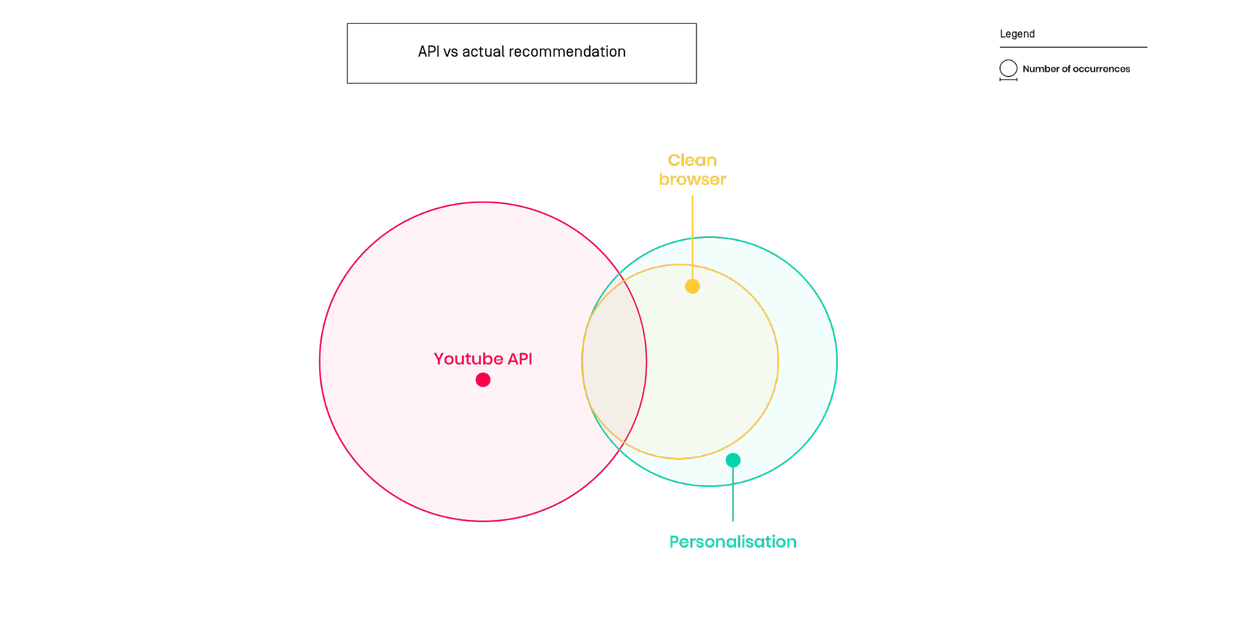
\includegraphics[width=\textwidth]{figures/api}}
	\caption{La differenza tra i video raccomandati da Youtube restituiti dalle API ufficiali e quelli ricevuti da gruppi di utenti con un browser senza cronologia (clean browser) e altri con profili molto utilizzati (personalized).}
	\label{fig:api}
\end{figure}

Sarebbe interessante, in successivi campionamenti, utilizzare le tecniche e i software sopracitati per verificare se i valori di odio riscontrati con le nostre analisi qui riportate, siano o no minori di quelli reali a causa della metodologia usata nella raccolta dati.

\section{Analizzare \textit{Big Data}: Digital labor e Turco Meccanico }
Lo sviluppo di nuove tecnologie e la parallela esponenziale crescita delle capacità di calcolo e di immagazzinamento di dati prodotto negli ultimi 20 anni ha dato luogo alla nascita dei \textit{big data}. Questo termine viene riferito a enormi dataset che includono "unstructured data" che richiedono analisi in tempo reale. Da una parte questo tipo di dati pone problemi su quali siano le migliori modalità di organizzazione e gestione dei dati, dall'altra è forirera di nuove opportunità per scoprire varibili nascoste e comprendere fenomeno da un nuovo punto di vista \citep{chen2014}.

Anche a livello di organizzazione del lavoro, questa trasformazione ha determinato dei cambiamenti rilevanti. La nascita della "gig-economy"  ha portato con sè nuove nuovi status per i lavoratori e nuove organizzazioni del lavoro definite "digital labor" \citep{stefano2016}. Sono nati le "crowd-sourced/micro-work platforms" e le "work-on-demand platforms". Le prime funzionano con "micro-tasks" che vengono svolti solo online e possono essere ad esmpio la classificazione di foto, o la revisione di contenuti online, come ad esempio viene fatto da Amazon Mechanical Turk. Il secondo tipo di piattaforme rende possibile l'incontro tra consumatori e lavoratori che svolgono mansioni fisiche come i guidatori di taxi nell'esempio classico di Uber \citep{floridi2020}. 

Il Turco Meccanico è un marchingegno costruito da Wolfgang Von Kempelen alla fine del 18° secolo per impressionare la regina Maria Teresa d'Austria. Questo oggetto raprresentava una persona dalla fattezze turche ed era apparentemente in grado di giocare a scacchi in modo magistrale e in modo del tutto automatizzato. All'interno però nascondeva una vera persona, probabilmente di bassa statura, che manovrava la struttura e creava l'illusione di automazione [Fig. \ref{fig:turco}]. Da questa crezione Amazon ha preso il nome per il suo sito di \textit{micro-work}, suggerendo appunto che algoritmi di \textit{machine learning} che richiedono enormi dataset categorizzati per arrivare a prestazioni a volte superiori a quelle umane, in realtà siano basati sul micro-lavoro svolto da miglia se non milioni di persone sparse per il mondo.  
\begin{figure}
	\centering
	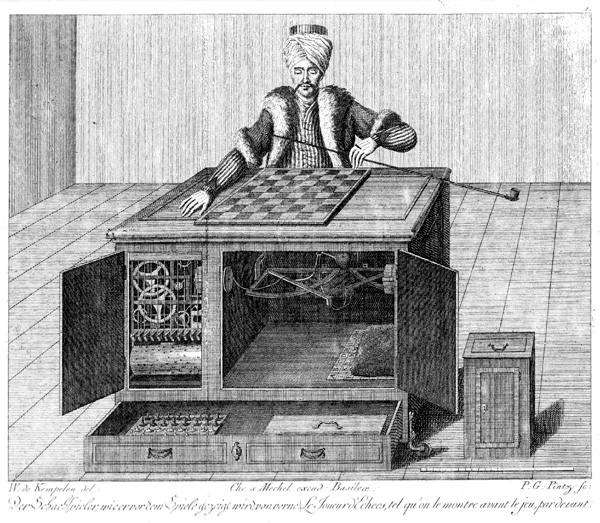
\includegraphics[width=\textwidth]{figures/turco}
	\caption{Una rappresentazione del Turco Meccanico probabilmente disegnata dal suo creatore Kempelen}
	\label{fig:turco}
\end{figure}

Il presente studio, come quello di Amnesty International, si è confrontato con i \textit{big data}, e ha deciso di impiegare una metodologia di valutazione di questi dati assimilabile ai \textit{micro-tasks} delle \textit{crowd-sourced/micro-work platforms}. Concretamente, sono state utilizzate delle piattaforme digitiali basate su \textit{cloud} per distribuire un grande numero di contenuti facenti parte di un unico progetto a vari ricercatori distribuiti in vari luoghi geograficamente anche molto lontani. 

La differenza principale tra il presente lavoro di codifica e piattaforme come quella di Amazon risiede nel ruolo del valutatore: non si parla in questo caso di lavoratori e lavoratrici che svolgono "lower-skill tasks", ma di ricercatori e ricercatrici attentamente istruit* allo svolgimento di un compito tutt'altro che facile o intuitivo come l'applicazione di categorie come \textit{hate speech} e \textit{negative campaign}. L'altra fondamentale differenza risiede nei diversi obiettivi: nel nostro caso la finalità ultima è una ricerca scientifica e non il profitto, obiettivo tanto di chi ha realizzato la ricerca che di chi ha aiutato con le codifiche. Nel caso della ricerca "Barometro dell'odio" i \textit{coders} si descrivono come attivisti e hanno un obiettivo sia politico che di ricerca, ma la sostanza rimane fondamentalmente diversa da quella di aziende come Amazon.

Benchè quindi i due processi partano dalla stessa problematica (l'utilizzo di \textit{big data}) e utilizzino la stessa tecnica (\textit{micro-work} \textit{cloud}), differiscono per tipo di compito svolto (qualificato, che necessità di studio rispetto a compiti semplici) e per obiettivi (ricerca e non profitto). Queste metodologie simili risultano bene descritte solo dal punto di vista dell'evolzione delle forme di lavoro e poco dal punto di vista dell'evoluzione delle tecniche di ricerca, ma risultano fondamentali per poter beneficiare delle più recenti sviluppi tecnologici in un ambito come nell'altro.

La costruzione di \textit{tool} in grado di faicilitare questo tipo di lavoro cooperativo all'interno delle università potrebbe risultare una sfida cruciale per il futuro delle ricerche basate sull'analisi qualitativa e manuale di \textit{big data}, la costituzione di reti di collaborazione tra ricercatrici e ricercatori in quest'ottica potrebbe favorire le analisi in molti ambiti del sapere, diventandone un requisito fondamentale, una condizione \textit{sine qua non}.